\section{Bandpass Sampling}
\label{Chap:Bandpass_Sampling}
\begin{frame}[t]{Chapter \autoref{Chap:Bandpass_Sampling}}
\tableofcontents[sections= \value{section}]
\end{frame}



\subsection{Introduction}

\begin{frame}[t,allowframebreaks]{Introduction and Motivation}

\begin{itemize}

\item Based on Paper of \cite{Sub_Nyquist_sampling}\footnotemark and textbooks \cite{DSP_Proakis}, \cite{DSP_practical_approach}, and \cite{book_understanding_dsp}
\footnotetext[1]{Sub-Nyquist Sampling,Bridging theory and Practice, By Moshe Mishali and Yonina C. Eldar,IEEE SIGNAL PROCESSING MAGAZINE,NOVEMBER 2011}

\item By bandpass signals $\leftrightarrow$ amplitude spectrum isn't centered at 0 Hz \cite{book_understanding_dsp}

	\begin{itemize}
	\item Instead, the spectrum is centered at some frequency $f_{\text{center}} \, \neq \, 0$ Hz \cite{book_understanding_dsp}
	
	\item Such signals are encountered in RF application (communication and radar)
	\end{itemize}

\item An example of such signals is shown in figure \autoref{fig:Bandpass_Sampling:multiband_signals}

\newpage
\begin{figure}[ht]
\centering
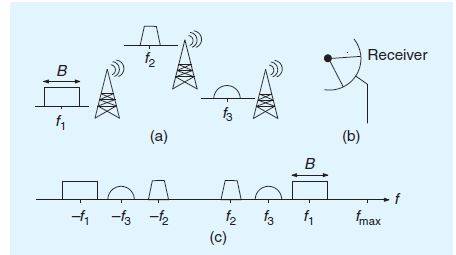
\includegraphics[scale = 0.4]{Figures/Bandpass_Sampling/multiband_signals}
\caption{Parts (a)–(c) show three RF transmissions with different carriers $f_i$. In (c), the receiver sees a multiband signal \cite{Sub_Nyquist_sampling}}
\label{fig:Bandpass_Sampling:multiband_signals}
\end{figure}

	\begin{itemize}
	\item The amplitude spectrum is centered at a center frequency $f_{\text{center}}$
	\end{itemize}


\end{itemize}

\end{frame}

\begin{frame}[t]{Parameters of a Bandpass Signal}

\begin{figure}[ht]
\centering
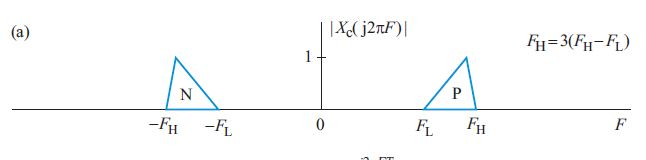
\includegraphics[scale = 0.4]{Figures/Bandpass_Sampling/bandpass_signal_example_2}
\caption{Amplitude Spectrum of a Bandpass Signal \cite{DSP_DimitrisManolakis}}
\label{fig:Bandpass_Sampling:bandpass_signal_example_2}
\end{figure}

\begin{itemize}

\item center frequency $f_{\text{center}}$
	
\item The bandwidth $B \, = \, f_{\text{high}} \, - \, f_{\text{low}} \, = \, f_{\text{upper}} \, - \, f_{\text{lower}} $ 
	 
\item Also any bandpass spectrum has a \textcolor{red}{positive and negative spectrum portion} since bandpass signals are reals signals
	 
\end{itemize}

\end{frame}


\begin{frame}[t]{Sampling a Bandpass Signals: Less than Nyquist rate}

\begin{itemize}

\item When we need to sample a bandpass signals, we could also apply the Nyquist theorem by setting $f_s \, = \, 2 \, \times \, f_{\text{upper}}$

\item However, $f_{\text{upper}}$ is usually big to any practical A/D converter

\item Instead, we can do sampling for such kind of signals in clever way by avoiding using such high frequencies


\item Advantages \cite{book_understanding_dsp}

	\begin{enumerate}
	\item Reduce \textcolor{red}{speed requirement of A/D converters} below that necessary in conventional low-pass sampling
	
	\item Reduce \textcolor{red}{amount of digital memory }necessary to capture a given time interval of a continuous signal
	\end{enumerate}


\item 2 methods to deal with sampling of such kind of signals:


	\begin{enumerate}
	\item Band-positioning
	
	\item Quadrature Sampling based on equivalent based band representation
	
	\end{enumerate}


\end{itemize}

\end{frame}


\subsection{Band positioning}
\begin{frame}[t]{Band positioning}

\begin{itemize}

\item What is band position ?

	\begin{itemize}
	\item It refers to the fractional number of bandwidths from the origin at which the lower band edge resides \cite{paper_bandpass_sampling_theory}.
	\end{itemize}

\item Unlike low-pass sampling, we are \textcolor{red}{interested in the signal bandwidth} rather by its highest frequency components

\item Instead of applying $F_s \geq \, 2 \, f_{\text{upper}}$, we will see that we can take $ 2 \, B \leq \, F_s \, \leq \, 4 \, B$

	\begin{itemize}
	\item Notice that we have gain allot by reducing $F_s$ from $ 2 \, f_{\text{upper}} \, \rightarrow \, [\,2 \, B \, ; \, 4 \, B \, ]$ because usually $f_{\text{upper}} >\, >\, B$
	
	\item Interesting thing that the range $2 \, B \leq \, F_s \, \leq \, 4 \, B$ implies that Nyquiste rate is always respected similar to the baseband case
	\end{itemize}

\end{itemize}

\end{frame}

\begin{frame}[t]{Integer Band positioning}

\begin{itemize}

\item We begin with a \textcolor{red}{special case} of \textcolor{red}{band positioning} technique known as \textcolor{red}{integer band positioning}

	\begin{itemize}
	\item $f_{\text{upper}}$ is an \textcolor{red}{integer multiple} of the \textcolor{red}{signal bandwidth} $B \, \leftrightarrow \, f_{\text{upper}} \, = \, K \, (f_{\text{upper}} \, - \, f_{\text{lower}}) \, = \, K \, B$ where $K \in \mathbb{N}$
	\end{itemize}


\item In this case, we can take $F_s \, = \, 2 \, B$ to sample this bandpass signal, and reconstruct without any distortion or aliasing

\item Ideal Interpolator (also known as \textcolor{red} {modulated interpolator}) formula in this case:

\begin{equation}
g_{\text{int}}(t) \, = \, \text{sinc}(B \, t) \, \text{cos}(2 \, \pi \, f_{\text{center}} \, t)
\end{equation}

\end{itemize}

\end{frame}


\begin{frame}[t]{Arbitrary band positioning}

\begin{itemize}
\item Now we move to a \textcolor{red}{more general case}, where  $f_{\text{upper}}$ isn't a multiple of the signal bandwidth $B$, a more general analysis is to be required


\item In this case, $F_s$ need to verify some  \textcolor{red}{constraints} translated by following \textcolor{red}{inequalities}:

\begin{equation}
\displaystyle\frac{2 \, f_{\text{upper}}}{k} \, \leq \, F_s \, \leq \, \displaystyle\frac{2 \, f_{\text{lower}}}{k \, - \, 1}
\end{equation}

\item In terms of $f_{\text{center}}$ and signal bandwidth $B$ we can write the above constraints as \cite{book_understanding_dsp}:

\begin{equation}
\displaystyle\frac{2 \, f_{\text{center}} \, + \, B}{k} \, \leq \, F_s \, \leq \, \displaystyle\frac{2 \, f_{\text{center}} \, - \, B}{k \, - \, 1}
\end{equation}

such that $f_{\text{center}} \, = \, \displaystyle\frac{f_{\text{lower}} \, + \, f_{\text{upper}}}{2}$


\end{itemize}

\end{frame}


\begin{frame}[t,allowframebreaks]{Graphical Interpretation}


\begin{itemize}

\item Graphical Interpretation:

\begin{figure}[ht]
\centering
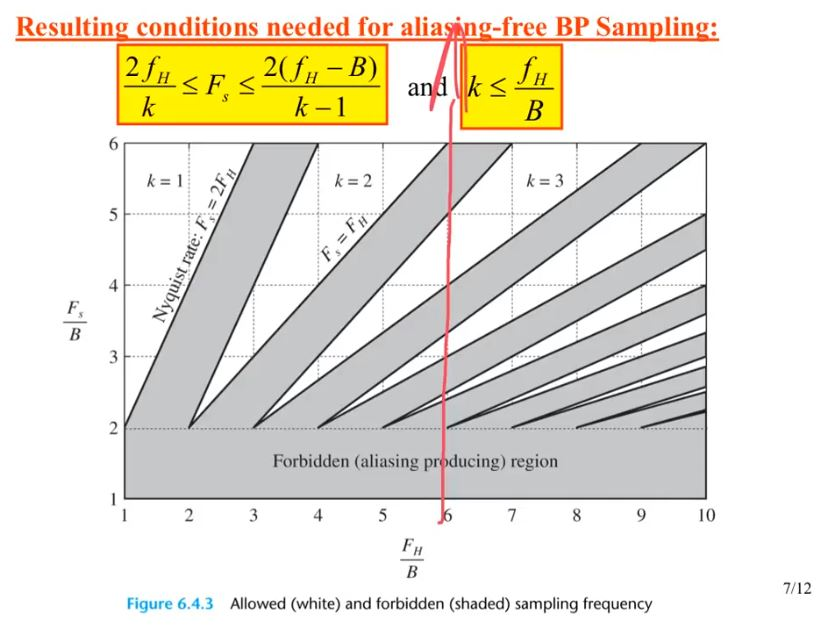
\includegraphics[scale = 0.3]{Figures/Sampling/bandpass_sampling_general_case_plots}
\caption{Bandpass sampling plot: $F_s$ function of $f_{\text{high}}$}
\label{fig:Sampling:bandpass_sampling_general_case_plots}
\end{figure}

	\item The plots are normalized over the bandwidth $B$, which makes plotting the equation more easy
	
	\item $k \, = \, 1$: we are operating on the standard Nyquiste rate
	
	
	\item if we have $\displaystyle\frac{f_{\text{high}}}{\text{ bandwidth}} \, = \, 6$, we can operate at multiple $k$: 1,2, 3 and 4 and even 5 (the higher $k$ the lower is $F_s$)
	
	\newpage
	\item However, we have to pay attention at $k \, = \, 5$
	
	\begin{figure}[ht]
\centering
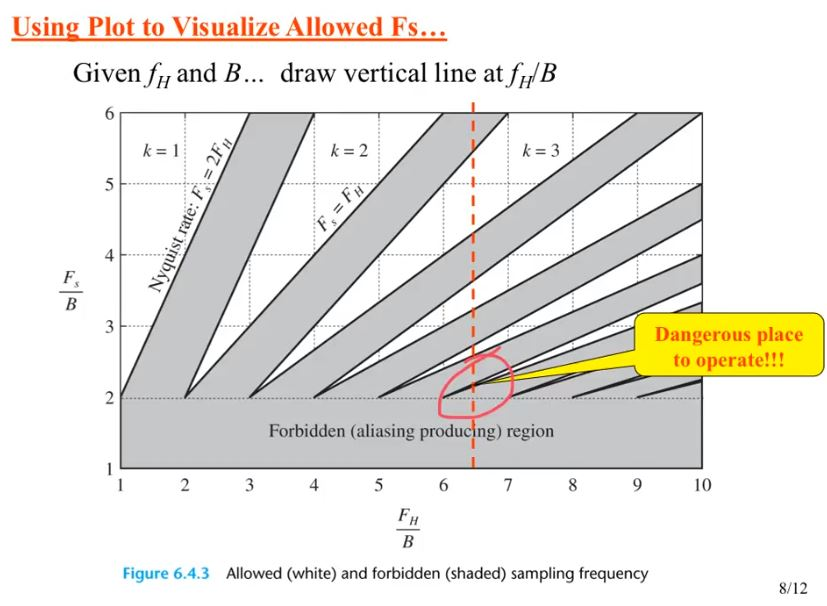
\includegraphics[scale = 0.3]{Figures/Sampling/bandpass_sampling_general_case_plots_2}
\caption{Bandpass sampling plot: dangerous area we need to pay attention from}
\label{fig:Sampling:bandpass_sampling_general_case_plots_2}
\end{figure}

	\item From this dangerous place, comes the idea of guard band shown in \autoref{fig:Sampling:bandpass_sampling_guard_bands}
	
	
	\begin{figure}[ht]
\centering
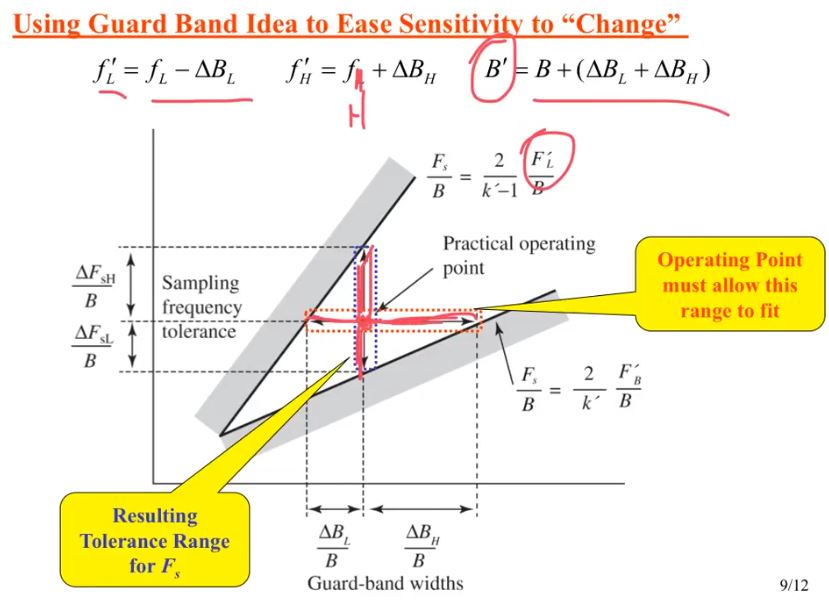
\includegraphics[scale = 0.3]{Figures/Sampling/bandpass_sampling_guard_bands}
\caption{Bandpass sampling plot:putting some guard bands}
\label{fig:Sampling:bandpass_sampling_guard_bands}
\end{figure}



\end{itemize}



\end{frame}


\subsection{Quadrature Sampling}
\begin{frame}[t,allowframebreaks]{Introduction In-phase and Quadrature Components of a Signal}

\begin{itemize}

\item \textcolor{red}{Before} we dive into what is called \textcolor{red}{qudarature sampling}, we begin by \textcolor{red}{explaining} what is so called \textcolor{red}{in-phase and quadrature representation (denoted by IQ) for a bandpass signal}

	\begin{itemize}
	\item These components will be used in quadrature sampling scheme
	\end{itemize}

\item From where the IQ components come from ?

\item Recall that when we have a bandpass signal, our target is to reduce the sampling rate $F_s$ and try to make as a function of the signal bandwidth $B$ rather than applying Nyquist rate directly (where it give us $F_s \, \geq \, 2 \, f_{\text{upper}}$)

	\begin{itemize}
	\item This what we have done in band positioning method
	\end{itemize}

\newpage
\item Another way to approach this problem, is to \textcolor{red}{shift the frequency spectrum} (say the postive part) and \textcolor{red}{centered about 0 Hz}, and make it a baseband signal
	
	\begin{itemize}
	\item In other words, we want to obtain an \textcolor{red}{equivalent low-pass signal} of the bandpass signal
	
	\item We do this because working with baseband representation is easier for DSP processing task
	
	\item This \textcolor{red}{equivalent low-pass signal} will contains the quadrature and in-phase component in which they will be used in bandpass signal representation
	\end{itemize}

\end{itemize}

\end{frame}


\begin{frame}[t]{Steps to be taken}

\begin{enumerate}

\item Derive the equivalent baseband representation of a bandpass signal

	\begin{itemize}
	\item This will give birth to IQ components
	\end{itemize}

\item Make the link between the bandpass signals and the in-phase and quadrature component

\item Use this new representation to do sampling

\item Reconstruction formula

\end{enumerate}


\end{frame}


\begin{frame}[t]{Steps to derive Equivalent Lowpass Signal for a Bandpass Signal}


\begin{figure}[ht]
\centering
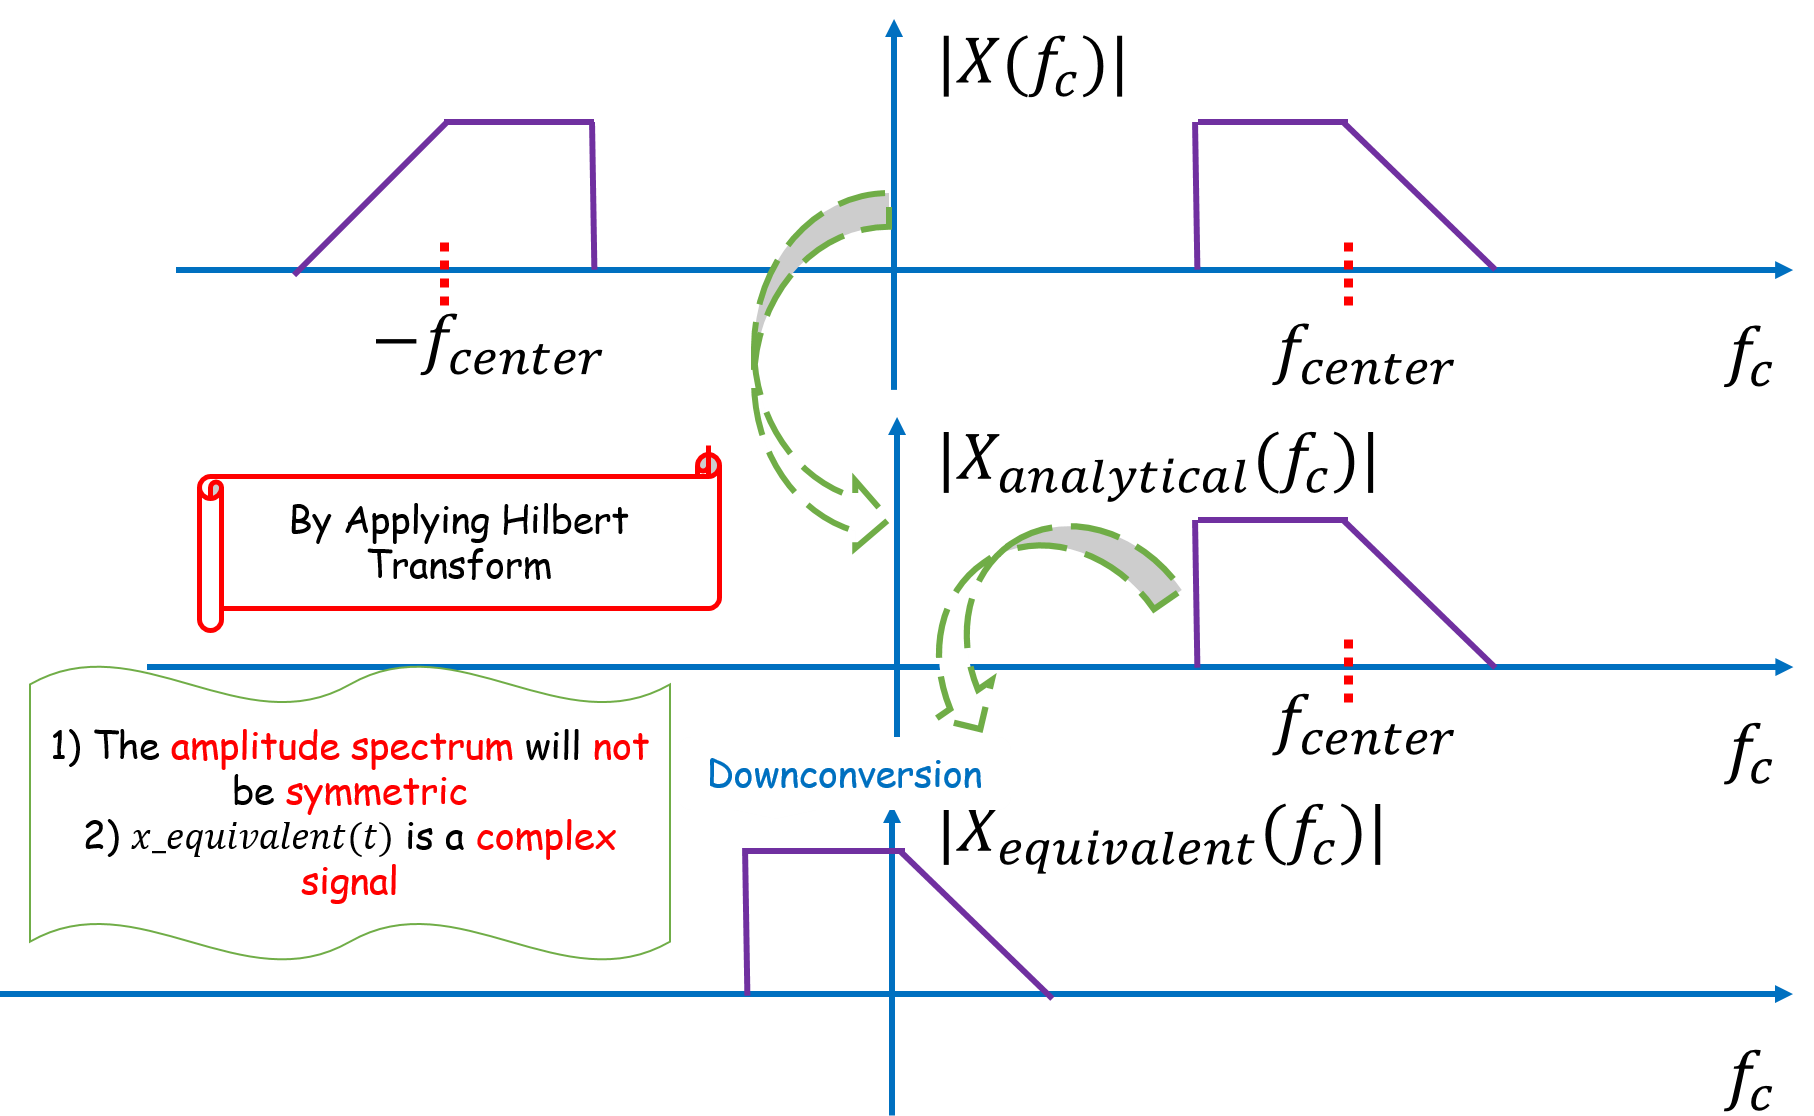
\includegraphics[scale = 0.35]{Figures/Bandpass_Sampling/equivalent_lowpass_signal_steps}
\label{fig:Bandpass_Sampling:equivalent_lowpass_signal_steps}
\end{figure}


\end{frame}


\begin{frame}[t,allowframebreaks]{Bandpass Signal Representation}

\begin{itemize}
	
\item \underline{Rule:}  Any \textcolor{red}{bandpass signal} can be written in terms of \textcolor{red}{in-phase and quadrature components} which are \textcolor{red}{complex baseband signals}
	
	
\item Sampling Each Component at a rate of $F_s$

\item Bandpass Signal Representation \cite{DSP_Proakis} \cite{paper_bandpass_sampling_theory}:

	\begin{equation}
\begin{array}{rcl}
x_{\text{band-pass}}(t) \, &=&\, \text{Amp}(t) \, \times \, \text{cos}\left(\, 2 \pi \, f_{\text{center}} \, t \, + \, \text{phase}(t) \,\right)\\ \\
&=&\, x_{\text{in-phase}}(t) \, \text{cos}\left( \, 2 \pi \, f_{\text{center}} \, t \,\right) \\
 && \, - \, x_{\text{quadrature}}(t) \, \text{sin}\left( \, 2 \pi \, f_{\text{center}} \, t \,\right)
\end{array}
\label{Eq:Sampling:based_band_general_form_time_domain_recap}
\end{equation}


\item In-phase and Quadrature Components:

	
	\begin{equation}
\begin{array}{rcl}
x_{\text{in-phase}}(t) \, &=& \, \text{Amp}(t) \, \times \, \text{cos}\left[\, \text{phase}(t) \, \right] \\ \\
x_{\text{quadrature}}(t) \, &=& \, \text{Amp}(t) \, \times \, \text{sin}\left[\, \text{phase}(t) \, \right] \\ \\
\end{array}
\label{Eq:Sampling:inpahse_quadrature_signals}
\end{equation}
	
	
\end{itemize}

\end{frame}


\begin{frame}[t,allowframebreaks]{Implementation}


\begin{figure}[ht]
\centering
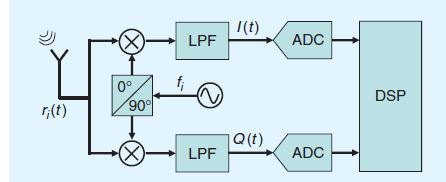
\includegraphics[width = 0.7\textwidth]{Figures/Sampling/I_Q_system}
\caption{A block diagram of a typical I-Q demodulator \cite{Sub_Nyquist_sampling}}
\label{fig:Sampling:I_Q_system}
\end{figure}

\begin{itemize}

\item The LPF is here due to high unwanted frequency components that we don't need them


\item Proofs: finish them on my initial report didn't have time to rewrite them from

\item Interpretation: Now we have 2 basedband signal (however remember that they are complex), and we can sample at a rate of  $F_s \, = \, B$ 

	\begin{itemize}
	\item But recall we have I and Q components
	
	\item So in total we have $F_s \, = \, 2 \, B$ 
	\end{itemize}

\item Application \cite{Sub_Nyquist_sampling}: This option is used in relay stations or regenerative repeaters
that decode the information I 1t 2, Q1t 2, use digital error correction algorithms, and then transform the signal back to high frequencies for the next transmission section
	
\end{itemize}
	
\end{frame}


\begin{frame}[t]{Band Positioning and IQ Comparison}

Note: to be put in a form of a table later

\begin{enumerate}

\item Band positioning:
	
	\begin{itemize}
	\item Can be applied directly to the signal $x(t)$ with no analog preprocessing hardware as in IQ
	
	\item But not suited for multiband signals
	\end{itemize}



\item IQ Demodulation

	\begin{itemize}
	\item Suitable for RF transmission which offers decoupling property of the dependency of the bandwidth of A/D on the maximal frequency of the input (like an RF transmitted signal) 
	
	
	\item Only in-band noise is inputted 
	\end{itemize}


\end{enumerate}


\end{frame}


\begin{frame}[t,allowframebreaks]{Integer band positioning}

\begin{itemize}



\item Thanks to the course of Dr.Mark Fowler, Binghmton University, State University of New York

	\begin{itemize}
	\item More pedagogical way to explain these concepts
	\end{itemize}



\begin{figure}[ht]
\centering
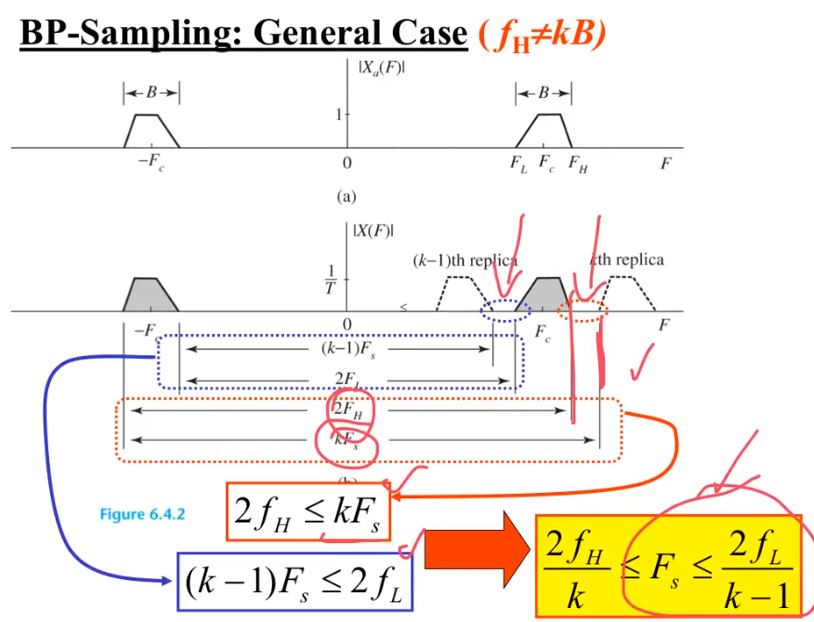
\includegraphics[width = 0.6\textwidth]{Figures/Sampling/bandpass_sampling_general_case_non_integer}
\caption{Bandpass sampling non integer case}
\label{fig:Sampling:bandpass_sampling_general_case_non_integer}
\end{figure}

\newpage
\item Equations:

\begin{equation}
\begin{array}{rcl}
\displaystyle\frac{2 \, f_{\text{high}}}{k} \, &\leq& \, F_s \,\, \, \, \leq \, \displaystyle\frac{2 \,\left( \,  f_{\text{high}} \, - \, \text{Bandwidth} \, \right)}{k \, - \, 1} \\ \\
k \, &\leq& \, \displaystyle\frac{2 \, f_{\text{high}}}{\text{Bandwidth}} 
\end{array}
\label{Eq:Sampling:bandpass_sampling_bounds}
\end{equation}

\item Graphical Interpretation:

Plotting equations (\ref{Eq:Sampling:bandpass_sampling_bounds}) give us plot shown in \autoref{fig:Sampling:bandpass_sampling_general_case_plots}.


\begin{figure}[ht]
\centering
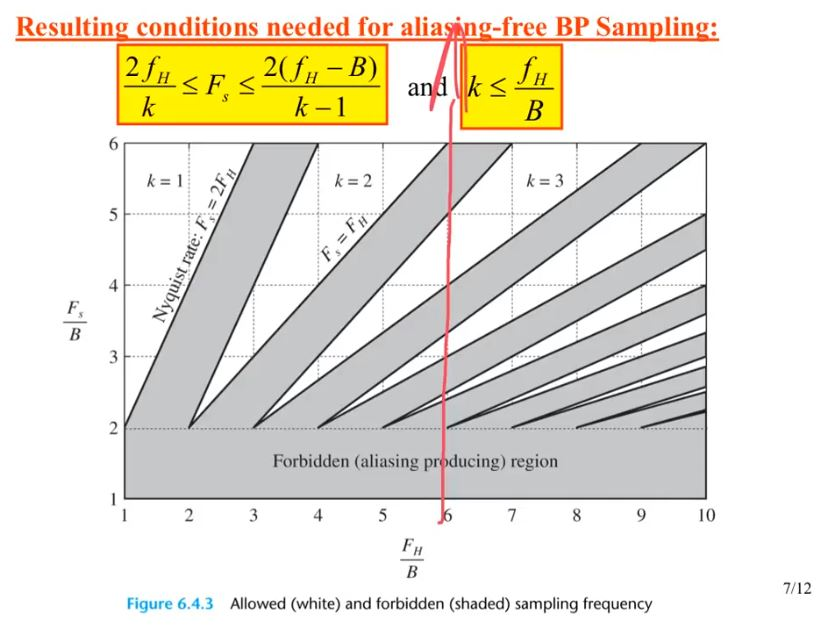
\includegraphics[width = 0.7\textwidth]{Figures/Sampling/bandpass_sampling_general_case_plots}
\caption{Bandpass sampling plot: $F_s$ function of $f_{\text{high}}$}
\label{fig:Sampling:bandpass_sampling_general_case_plots}
\end{figure}

	\begin{itemize}
	\item The plots are normalized over the bandwidth $B$, which makes plotting the equation more easy
	
	\item $k \, = \, 1$: we are operating on the standard Nyquiste rate
	
	
	\item if we have $\displaystyle\frac{f_{\text{high}}}{\text{ bandwidth}} \, = \, 6$, we can operate at multiple $k$: 1,2, 3 and 4 and even 5 (the higher $k$ the lower is $F_s$)
	
	\newpage
	\item However, we have to pay attention at $k \, = \, 5$
	
	\begin{figure}[ht]
\centering
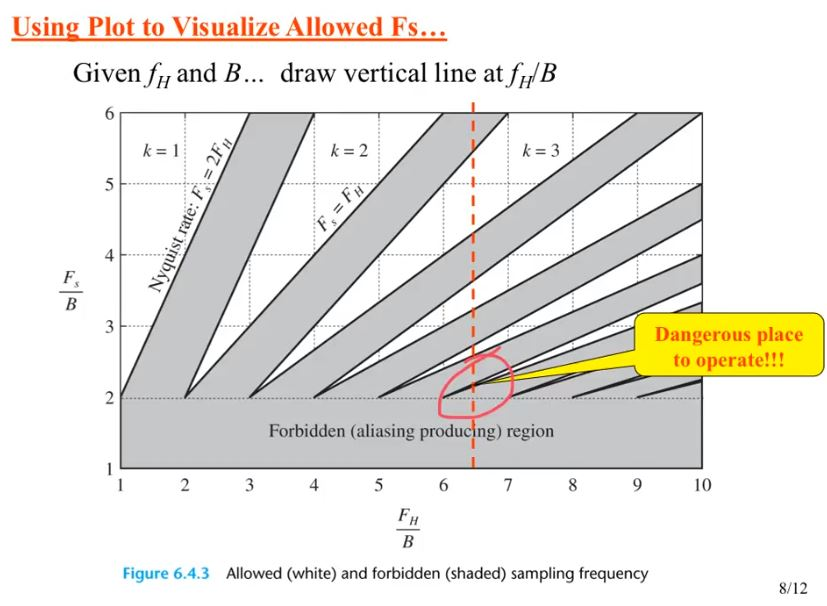
\includegraphics[width = 0.7\textwidth]{Figures/Sampling/bandpass_sampling_general_case_plots_2}
\caption{Bandpass sampling plot: dangerous area we need to pay attention from}
\label{fig:Sampling:bandpass_sampling_general_case_plots_2}
\end{figure}

	\item From this dangerous place, comes the idea of guard band shown in \autoref{fig:Sampling:bandpass_sampling_guard_bands}
	
	
	\begin{figure}[ht]
\centering
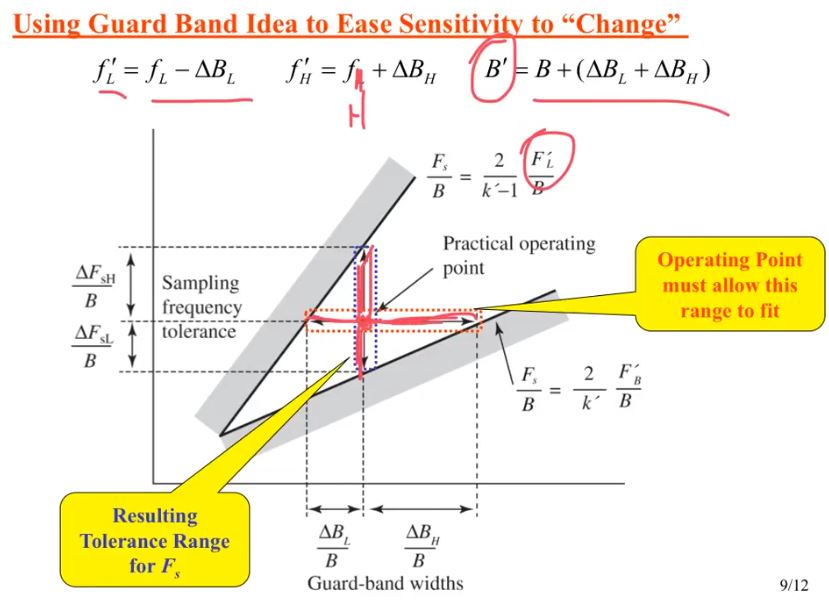
\includegraphics[width = 0.7\textwidth]{Figures/Sampling/bandpass_sampling_guard_bands}
\caption{Bandpass sampling plot:putting some guard bands}
\label{fig:Sampling:bandpass_sampling_guard_bands}
\end{figure}
	
	\end{itemize}



\end{itemize}


\end{frame}
